\documentclass[a4paper,10pt]{article}
\usepackage[utf8]{inputenc}
\usepackage{graphicx}
\usepackage{hyperref}
\usepackage{svg}
\usepackage{ngerman}

%opening
\title{Echtzeit und Betriebssysteme Praktikumsaufgabe 1}
\author{Louis Krumme}

\begin{document}

\maketitle

\section{Aufabe 1 - Teil 1}
\subsection{a) - Was bewirkt der Befehl?}
Der Befehl zählt mit `find .` alle Dateien im Aktuellen Verzeichnis auf. Diese Ausgabe wird mit `|` in `xargs` gepipet. `xargs` gibt die Dateien als Argumente von `grep` weiter. Somit hat `grep testString` als weitere Argumente alle Dateien und Ordner des akutellen Verzeichnissen. `grep` überpüft Muster, allerdings passt keine der Dateien oder Ordner auf das Muster `testString`. Wenn `grep` jetzt ein Verzeichnis auf ein Muster prüfen soll wird ein Fehler geworfen. Somit kommt die Ausgabe zustande, dass alle Verzeichnisse aus dem aktuellen Verzeichnis ausgegeben werden: \\

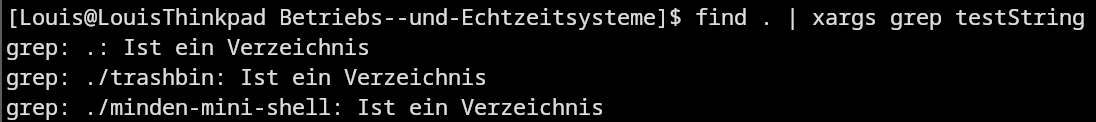
\includegraphics[width=1\textwidth]{befehl.png}

\subsection{b) Überprüfung von Pfadnamen}
Dateien:
\begin{enumerate}
 \item pathinfo.sh
\end{enumerate}
Ausgabe: \\
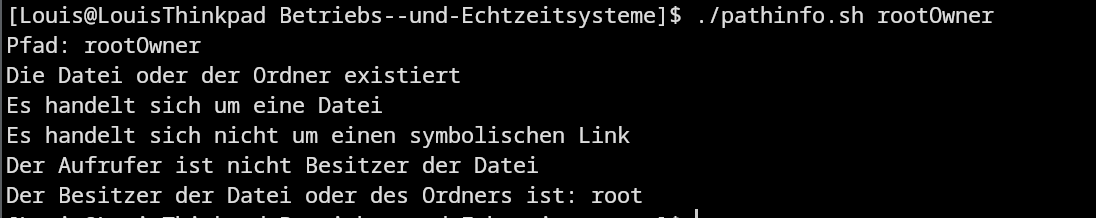
\includegraphics[width=1\textwidth]{pathinfo_ausgabe.png}

\subsection{c) Schleifen}
Dateien:
\begin{enumerate}
 \item pathinfo1c).sh
\end{enumerate}
Ausgabe:\\
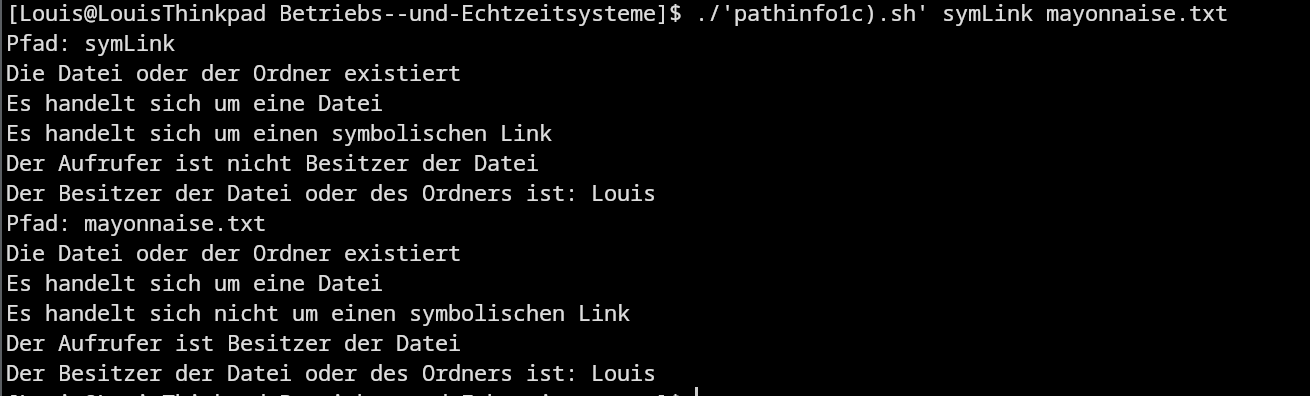
\includegraphics[width=1\textwidth]{pathinfo1c)_ausgabe.png} \\
Anmerkung: Der symbolische Link `symlink` zeigt auf `rootOwner`, dessen besitzer root ist. Der Besitzer von `symLink` ist Louis. Deswegen wird angegeben, dass der Aufrufer nicht der Besitzer ist, obwohl Aufrufer und Besitzer(von symLink) beide Louis sind.
\subsection{d) Auswahl}
Dateien:
\begin{enumerate}
 \item pathinfo1d).sh
\end{enumerate}
Ausgabe: \\
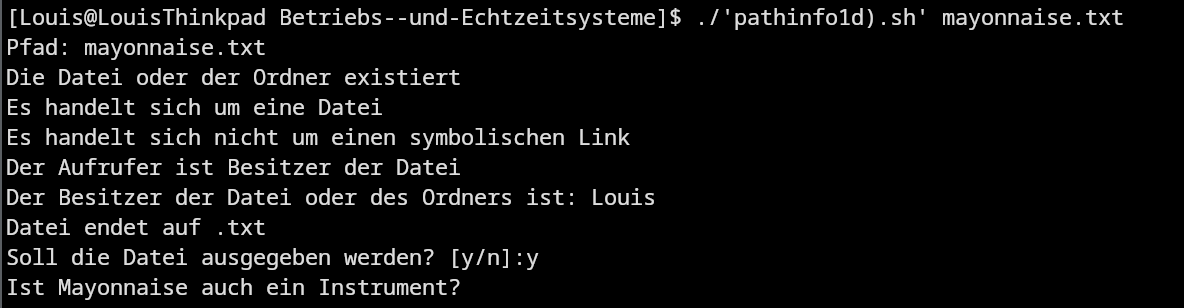
\includegraphics[width=1\textwidth]{pathinfo1d)_ausgabe.png}

\section{Teil 2 Papierkorb}
Datein:
\begin{enumerate}
 \item delete
 \item undelete
\end{enumerate}
Beides sind shell Skripte ohne `.sh` Endung, da die Befehle in der Aufgabe `delete` und `undelete` genannt wurden.\pagebreak

Ausgabe: \\ \\
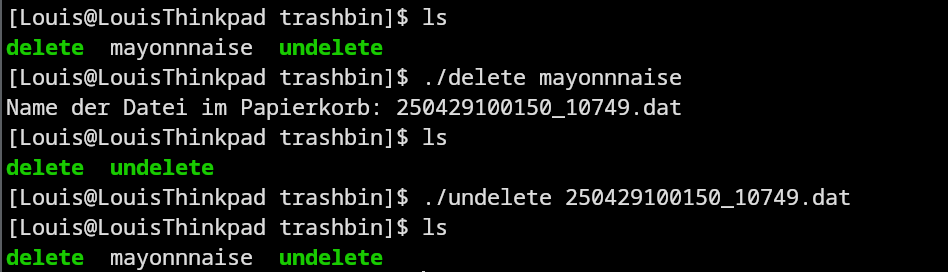
\includegraphics[width=1\textwidth]{trashbin_ausgabe.png}
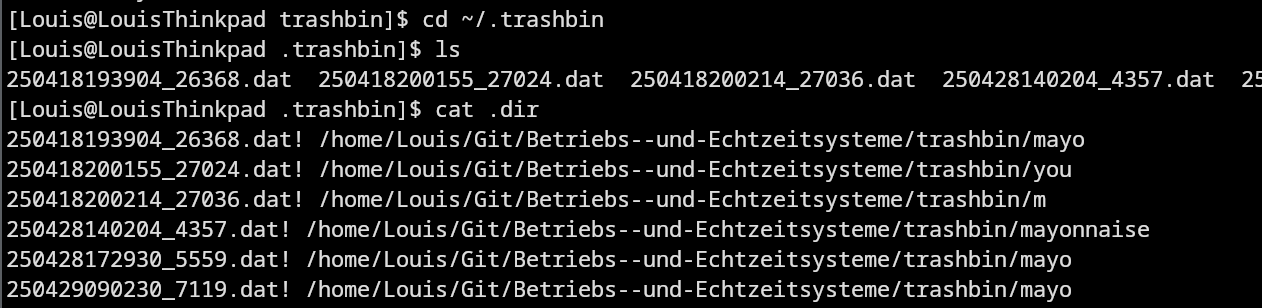
\includegraphics[width=1\textwidth]{trashbin_dir.png}

\section{Teil 3 Minden-Mini-Shell}
Dateien:
\begin{enumerate}
 \item main.c
 \item makefile
\end{enumerate}
Ausgabe: \\\\
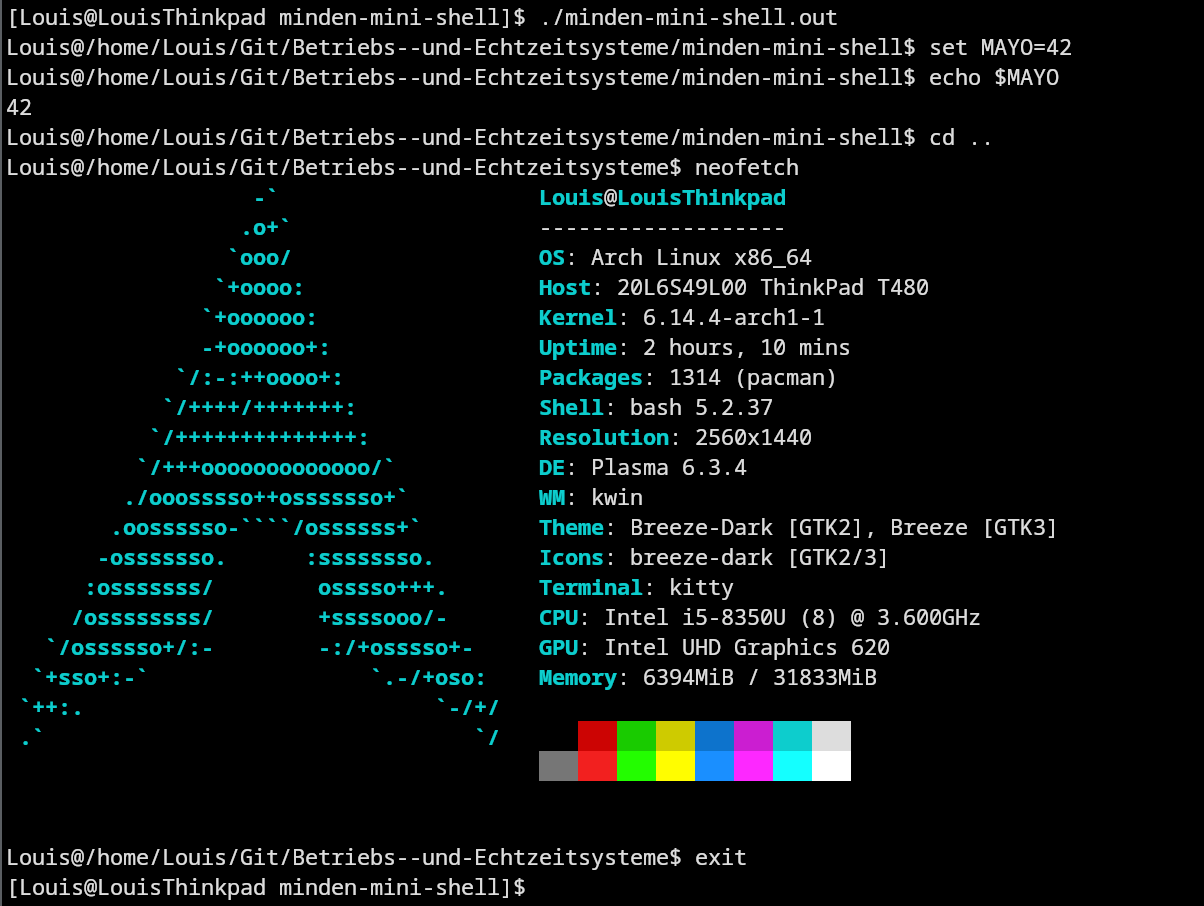
\includegraphics[width=1\textwidth]{minden-mini-shell_ausgabe.png}

\end{document}
